
In large scale variable screening studies, we would like to find suitable designs such that combinations of the dimensionality $p$, sparsity $\beta$, and signal sizes $r$ of the problem land in the desirable region of discovery, as predicted by the results in Section \ref{sec:chisq-boundaries}.

In practice, however, not all three of the parameters $(p, \beta, r)$ can be manipulated.
In particular, the problem dimensions and sparsity levels are usually determined by the underlying physical process.
In the GWAS example, the number of genomic marker locations is determined by the design of the chip used for sequencing, while the number of relevant genomic locations is a consequence of the biological process.
Therefore, in order to achieve a desired level of error control, one can only hope to influence the statistical signal sizes.

We discuss in this section how to attain the necessary statistical signal sizes in the case of association tests on 2-by-2 contingency tables, and clarify the relationship between statistical signal sizes and odds ratios in these tests.

\subsection{Odds ratios and statistical power}
\label{subsec:odds-and-power}

Although the non-centrality parameter $\lambda$ serves as a natural parameter for signal sizes in chi-square (and other omnidirectional) tests, its meaning is perhaps not as transparent.
A question frequently asked by practitioners is how signal sizes relate to odds ratios, commonly referred to as effect sizes in association tests.

Consider a 2-by-2 multinomial distribution with marginals probabilities $(\phi_1, \phi_2)$ and $(\theta_1, \theta_2)$, where $\phi_1 + \phi_2 = 1$ and $\theta_1 + \theta_2 = 1$.
\begin{center}
    \begin{tabular}{cccc}
    \hline
    & \multicolumn{2}{c}{Genotype} \\
    \cline{2-3}
    Probabilities & Variant 1 & Variant 2 & Total by phenotype \\
    \hline
    Cases & $\mu_{11}$ & $\mu_{12}$ & $\phi_1$ \\
    Controls & $\mu_{21}$ & $\mu_{22}$ & $\phi_2$ \\
    Total by genotype & $\theta_1$ & $\theta_2$ & 1 \\
    \hline
    \end{tabular}
\end{center}
The odds ratio is defined as the ratio of the phenotype frequencies between the two genotype variants,
\begin{equation} \label{eq:odds-ratio}
    \text{R} := \frac{\mu_{11}}{\mu_{21}}\Big/\frac{\mu_{12}}{\mu_{22}}
    = \frac{\mu_{11}\mu_{22}}{\mu_{12}\mu_{21}}.
\end{equation}
The multinomial distribution is fully parametrized by the trio $(\theta_1, \phi_1, R)$.
Independence between the genotypes and phenotyes would imply an odds ratio of zero, and hence
$$
\mu_{jk} = \phi_j\theta_k, \quad \text{for all }j,k \in\{1,2\}.
$$
When data are sampled from the multinomial distribution, the chi-square test defined in \eqref{eq:chisq-statistic} is asymptotically equivalent to tests including, e.g., the likelihood ratio test and Welch's t-test, both in terms of level and power \cite{ferguson2017course,gao2019upass}.

Specifically, with a sequence of local alternatives $\mu^{(1)}, \mu^{(2)}, \ldots$, such that $\sqrt{n}(\mu^{(n)}_{jk} - \phi_j\theta_k)$ converges to a constant table $\delta = (\delta_{jk})$, the aforementioned test statistics converge in distribution to the non-central chi-squared distribution with non-centrality parameter 
$$\lambda = \sum_{j=1}^2 \sum_{k=1}^2 {\delta_{jk}^2}/{(\phi_j\theta_k)}.$$
Therefore, for large samples from a fixed distribution $\mu$, the statistics would be well approximated by a $\chi^2_\nu(\lambda)$ distribution, where $\nu=1$ and
\begin{equation} 
    \lambda := n\sum_{j=1}^2 \sum_{k=1}^2 \frac{(\mu_{jk} - \phi_j\theta_k)^2}{\phi_j\theta_k}.
\end{equation}
Since $\lambda$ is linear in the number of samples $n$, we define 
\begin{equation} \label{eq:signal-size-chisq}
    w^2:=\lambda/n
\end{equation} 
as the signal size per sample.
Power of association tests at $\alpha$ level is approximately $\P[\chi^2_{\nu}(\lambda)>\chi^2_{\nu,\alpha}]$, where $\chi^2_{\nu,\alpha}$ is the upper $\alpha$-quantile of a central Chi-squared distribution.
Power calculations would therefore only depend on the distributions through $\lambda=nw^2$, and statistical power is increasing in the signal sizes per sample $w^2$.
The relationship between the $w^2$ and the odds ratio $\text{R}$ is characterized in the following proposition.

\begin{proposition} \label{prop:signal-size-odds-ratio}
Consider 2-by-2 multinomial distribution with marginals $(\phi_1, \phi_2)$ and $(\theta_1, \theta_2)$.
Let signal size $w^2$ be defined as in \eqref{eq:signal-size-chisq}, and odds ratio $\text{R}$ be defined as in \eqref{eq:odds-ratio}. 
Then we have $w^2 = 0$ if $R=1$, and
\begin{equation} \label{eq:signal-size-odds-ratio}
    w^2(\text{R}) =
    \frac{1}{4A(\text{R}-1)^2}\left(B+CR-\sqrt{(B+CR)^2-4A(R-1)^2}\right)^2,
\end{equation}
if $R\neq1$, and $R>0$, 
with constants $A = \phi_1\theta_1\phi_2\theta_2$, $B = \phi_1\theta_1+\phi_2\theta_2$, and $C = \phi_1\theta_2+\phi_2\theta_1$.
\end{proposition}

We illustrate Relation \eqref{eq:signal-size-odds-ratio} for selected values of marginals $\theta_1$ and $\phi_1$ in Figure \ref{fig:signal-vs-odds}.
Notice that while the odds ratio $R$ can be unbounded for any arbitrary marginal distributions, the signal sizes $w^2$ are bounded from above by constants that depend only on the marginals $\phi_1$ and $\theta_1$.
This is quantified in the next corollary.

\begin{figure}
      \centering
      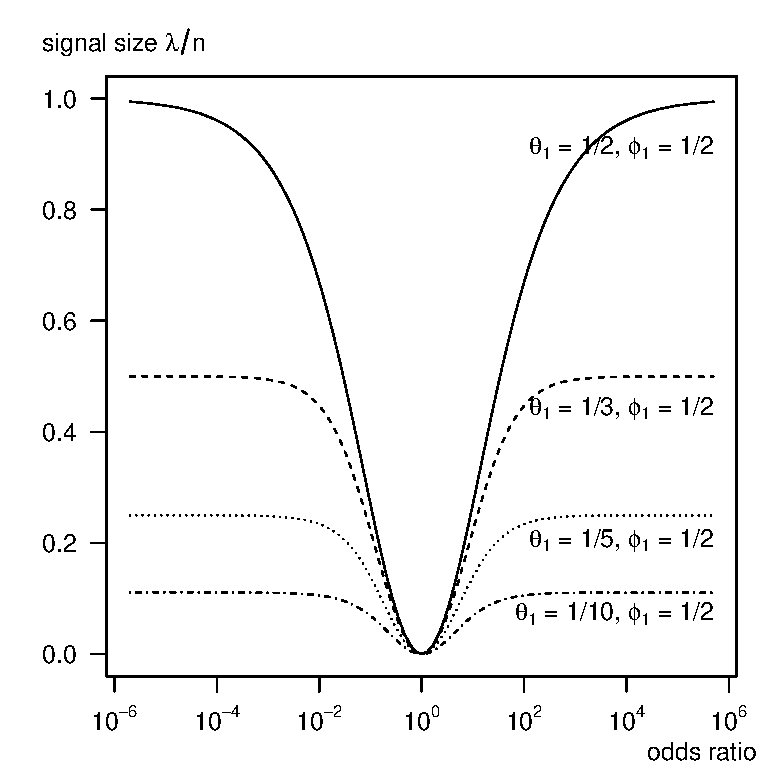
\includegraphics[width=0.49\textwidth]{./singal-vs-odds-p05}
      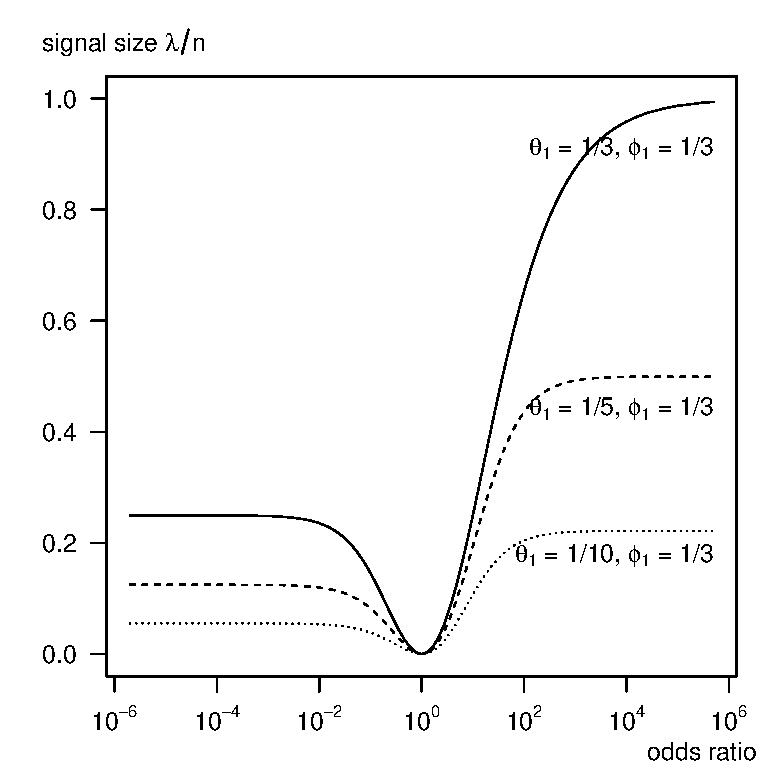
\includegraphics[width=0.49\textwidth]{./singal-vs-odds-p0333}            
      % 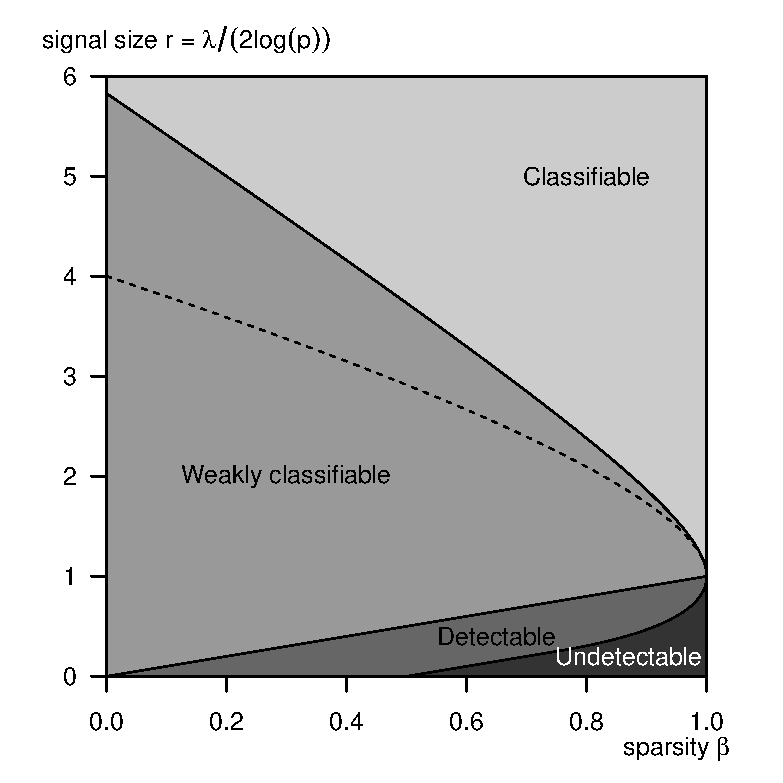
\includegraphics[width=0.35\textwidth]{./phase_diagram_chisquared.eps}
      \caption{Signal size in chi-square tests as functions of odds ratio in 2-by-2 multinomial distributions, for selected marginal probabilities; see Relation \eqref{eq:signal-size-odds-ratio} in Proposition \ref{prop:signal-size-odds-ratio}.
      For fixed marginal distributions, extreme odds ratios imply stronger signals at a given sample size.
      However, the signal sizes are bounded above by constants that depend on the marginal distributions; see Relation \eqref{eq:signal-size-upper-bound}.
      % Unbalanced marginal distributions -- or rare variants -- lead to smaller signal sizes at a given odds ratio.
      } 
      \label{fig:signal-vs-odds}
\end{figure}

\begin{corollary} \label{cor:signal-limits-OR}
The signal size as a function of the odds ratio $w^2(R)$ is decreasing on $(0,1)$ and increasing on $(1,\infty)$, with limits
\begin{equation} \label{eq:signal-size-upper-bound-1}
    \lim_{\text{R}\to0_+} w^2(\text{R}) = \min\left\{\frac{\phi_1\theta_1}{\phi_2\theta_2}, \frac{\phi_2\theta_2}{\phi_1\theta_1}\right\},
\end{equation}
and
\begin{equation} \label{eq:signal-size-upper-bound-2}
    \lim_{\text{R}\to+\infty} w^2(\text{R}) = \min\left\{\frac{\phi_1\theta_2}{\phi_2\theta_1}, \frac{\phi_2\theta_1}{\phi_1\theta_2}\right\}.
\end{equation}
\end{corollary}


\subsection{Rare variants and the optimal study design}
\label{subsec:optimal-design} 


We make the important distinction here between the marginal distributions of genotypes and phenotypes \emph{in subjects of the study}, versus the marginal distributions \emph{in the general population}.
Throughout this paper marginal distributions refer to the quantities \emph{in the study}.
As we will see in Section \ref{subsec:odds-and-power}, only the quantities in the study are relevant for statistical power, while quantities in the population do not play a role.

Typically in a genetic study, the marginal distribution of the phenotypes can be pre-determined.
That is, we are able to decide on the number of recruited subjects in cases and controls.
In contrast, the marginal distribution of the genotypes in the study are typically unknown a priori. 
On the other hand, the conditional distributions of the genetic variants in the healthy control groups are sometimes known.
We will see in Section \ref{subsec:optimal-design} that this information on the conditional distributions will allow us to determine the optimal proportion of cases versus controls in a study.


While the marginal distributions of alleles $(\theta_1, \theta_2)$ are often unknown before collecting the data, their conditional distributions in the healthy control group can sometimes be estimated from prior studies.
We denote the conditional frequency of the first allele among the subjects in the control group as
$$
f := \mu_{21} / \phi_2.
$$
Since we can always relabel the variants, we may assume without loss of generality that the first variant is associated with an increased risk of disease, and is henceforth referred to as the risk allele.
We shall also refer to a risk allele with very low frequency in the control group (i.e., $f\approx 0$) as a rare variant.

Just as the multinomial distribution is fully parametrized by the marginals and odds ratio  $(\theta_1, \phi_1, R)$, it can also be fully described by the conditional frequency of allele in the control group $f$, proportion of cases in the study $\phi_1$, and the odds ratio $R$.

\begin{center}
    \begin{tabular}{cccc}
    \hline
    & \multicolumn{2}{c}{Genotype} \\
    \cline{2-3}
    Probabilities & Variant 1 & Variant 2 & Total by phenotype \\
    \hline
    Cases & $\frac{\phi_1fR}{(fR+1-f)}$ & $\frac{\phi_1(1-f)}{(fR+1-f)}$ & $\phi_1$ \\
    Controls & $f(1-\phi_1)$ & $(1-f)(1-\phi_1)$ & $1-\phi_1$ \\
    \hline
    \end{tabular}
\end{center}

Proposition \ref{prop:signal-size-odds-ratio} may then be re-stated in terms of the new trio $(f, \phi_1, R)$.

% Note that all these quantities refer to what is in the study, and differ from their counterparts in the general population.

\begin{corollary} \label{cor:signal-size-odds-ratio-conditional-frequency}
In the 2-by-2 multinomial distribution with marginals $(\phi_1, \phi_2 = 1-\phi_1)$, and conditional distribution of the variants in the control group $(f, 1-f)$,
Relation \eqref{eq:signal-size-odds-ratio} holds with $\theta_1 = {\phi_1fR}/{(fR+1-f)} + f(1-\phi_1)$ and $\theta_2 = 1-\theta_1$.
\end{corollary} 

